%------------------------------------------------------------------------------
% Template file for the submission of papers to IUCr journals in LaTeX2e
% using the iucr document class
% Copyright 1999-2013 International Union of Crystallography
% Version 1.6 (28 March 2013)
%------------------------------------------------------------------------------

\documentclass[preprint]{iucr}              % DO NOT DELETE THIS LINE
\usepackage{amssymb}
\usepackage[fleqn]{amsmath}
\usepackage{graphicx}
\usepackage{tabularx}
\usepackage{booktabs}
\usepackage{longtable}
\usepackage{array}
\usepackage{color}
\usepackage{url}
\usepackage{makecell}
\usepackage{tikz}
\usepackage[outdir=./]{epstopdf}

\hyphenation{Niggli}
\def\mathbi#1{\textbf{\em #1}}
\numberwithin{equation}{section}

\renewcommand{\cellalign}{l}
\renewcommand{\cellgape}{\Gape[4pt]}

% lca IUCr id IUCr6401
% HJB IUCr id IUCr6484
% lca ORCID  0000-0002-4451-1641
% HJB ORCID 0000-0002-0517-8532

% Crystallographic space macros
\newcommand{\HVI}{\ensuremath{\mathbf{H}^{6}}}
\newcommand{\GVI}{\ensuremath{\mathbf{G}^{6}}}
\newcommand{\SVI}{\ensuremath{\mathbf{S}^{6}}}
\newcommand{\PIII}{\ensuremath{\mathbf{P}^{3}}}
\newcommand{\FIII}{\ensuremath{\mathbf{F}^{3}}}
\newcommand{\BIV}{\ensuremath{\mathbf{B}^{4}}}
\newcommand{\CIII}{\ensuremath{\mathbf{C}^{3}}}
\newcommand{\RIII}{\ensuremath{\mathbb{R}^{3}}}

% Unit cell vector macros
\newcommand{\va}{\ensuremath{\mathbf{a}}}
\newcommand{\vb}{\ensuremath{\mathbf{b}}}
\newcommand{\vc}{\ensuremath{\mathbf{c}}}

% Scalar/subscript macros
\newcommand{\scalar}[1]{\ensuremath{#1}}
\newcommand{\scalarsub}[2]{\ensuremath{#1_{#2}}}

%-------------------------------------------------------------------------
% Information about journal to which submitted
%-------------------------------------------------------------------------
\journalcode{A}              % Indicate the journal to which submitted
%   A - Acta Crystallographica Section A
%   B - Acta Crystallographica Section B
%   J - Journal of Applied Crystallography
%   M - IUCrJ

\makeatletter
\font\dummyft@=dummy \relax
\makeatother


\begin{document}                  % DO NOT DELETE THIS LINE
	
	%-------------------------------------------------------------------------
	% The introductory (header) part of the paper
	%-------------------------------------------------------------------------
	
	\begin{center}
		{\LARGE \emph{\today}} \\
	\end{center}
	
	\title{Niggli Reduction Reconsidered}
	\shorttitle{Niggli Reduction Reconsidered}
	
	\cauthor[a]{Lawrence C.}{Andrews}{larry6640995@gmail.com}{}
	\author[a]{Herbert J.}{Bernstein}
	
	\aff[a]{Ronin Institute for Independent Scholarship 2.0, USA}
	
	\shortauthor{Andrews and Bernstein}
	
	\keyword{Niggli reduction}
	\keyword{metric tensor}
	\keyword{lattice}
	\keyword{unit cell}
	\keyword{\GVI}
	\keyword{trace minimization}
	
	\maketitle                        % DO NOT DELETE THIS LINE
	
	
	\begin{abstract}
		Niggli reduction of a unit cell is conventionally described as a
		sequence of conditional steps enforcing inequalities on the components
		of the metric tensor in \GVI{}. We argue that the essential geometric
		content of Niggli reduction is the minimization of
		$\mathrm{Tr}(\mathbf{G}) = g_1 + g_2 + g_3 = a^2 + b^2 + c^2$,
		the sum of squared edge lengths, followed by secondary conditions that
		select a unique canonical representative from among all cells sharing
		the minimum trace. This reframing clarifies the termination argument
		of \citeasnoun{Krivy1976}, whose case analysis is shown to be
		implicitly a trace-minimization argument. The distinct causes of
		infinite loops in floating-point implementations are enumerated, and
		the treatment of \citeasnoun{grosse2004numerically} is examined in
		this light. Multiple distinct cells can share the same minimum trace
		value, as illustrated by example; Niggli's secondary conditions are
		essential precisely because of this degeneracy.
	\end{abstract}
	
	
	\section{Introduction}
	
	Niggli reduction \cite{Niggli1928} produces a canonical primitive unit
	cell. The computational algorithm of \citeasnoun{Krivy1976} is widely
	used for this purpose.
	
	The conventional description of Niggli reduction is procedural: a
	sequence of steps that enforce inequalities on the components of the
	metric tensor in \GVI{}. Here we describe Niggli reduction as
	minimization of a single quantity, $\mathrm{Tr}(\mathbf{G}) =
	g_1 + g_2 + g_3$, followed by secondary conditions that select a
	unique cell from among those sharing the minimum trace. To our
	knowledge this description does not appear in the literature.
	Section~\ref{sec:history} gives the historical background.
	Section~\ref{sec:g6} defines \GVI{}.
	Section~\ref{sec:trace} develops the trace-minimization description.
	Section~\ref{sec:loops} enumerates the causes of infinite loops in
	floating-point implementations and examines \citeasnoun{grosse2004numerically}.
	Section~\ref{sec:examples} gives examples.
	Section~\ref{sec:summary} is the summary.
	
	
	\section{Historical Background}
	\label{sec:history}
	
	Niggli reduction has its mathematical roots in the theory of positive
	definite ternary quadratic forms. As noted by \citeasnoun{Roof1967},
	the conditions defining a reduced cell descend from the work of
	Eisenstein \cite{Eisenstein1851}, who established criteria for a
	canonical reduced form of a positive definite ternary quadratic ---
	precisely the object represented by the metric tensor in \GVI{}.
	Niggli \cite{Niggli1928} applied these ideas to crystallographic unit
	cells, adding the ordering and sign-consistency conditions needed to
	select a unique canonical representative.
	
	The first practical algorithm implementing Niggli's conditions was given
	by \citeasnoun{Krivy1976}. Numerical stability issues in that algorithm
	were subsequently analyzed by \citeasnoun{grosse2004numerically}, who
	proposed modified procedures to improve robustness in floating-point
	computation. A detailed geometric analysis of the Niggli-reduced region
	in \GVI{} and its boundaries is given in \citeasnoun{Andrews2014}.
	
	
	\section{The \GVI{} Representation}
	\label{sec:g6}
	
	The metric tensor of a unit cell with basis vectors $\va, \vb, \vc$
	is the $3 \times 3$ symmetric positive definite matrix
	
	\begin{equation}
		\mathbf{G} = \begin{pmatrix}
			g_1      & g_6/2   & g_5/2 \\
			g_6/2   & g_2      & g_4/2 \\
			g_5/2   & g_4/2   & g_3
		\end{pmatrix},
		\label{eq:metrictensor}
	\end{equation}
	
	\noindent where
	\begin{equation}
		\begin{aligned}
			g_1 &= a^2, \quad g_2 = b^2, \quad g_3 = c^2, \\
			g_4 &= 2bc\cos\alpha, \quad g_5 = 2ac\cos\beta, \quad g_6 = 2ab\cos\gamma.
		\end{aligned}
		\label{eq:g6components}
	\end{equation}
	
	\noindent The six-component vector
	\begin{equation}
		\mathbf{g} = (g_1, g_2, g_3, g_4, g_5, g_6)
		\label{eq:g6vector}
	\end{equation}
	defines a point in \GVI{} \cite{Andrews2014}. Note that \citeasnoun{Gruber1973} introduced the notation
	$A, B, C, \xi, \eta, \zeta$ for the same quantities, where
	$\xi, \eta, \zeta$ correspond to our $g_4, g_5, g_6$; this
	notation is also used by \citeasnoun{Krivy1976} and
	\citeasnoun{grosse2004numerically}.
	
	The trace of $\mathbf{G}$ is
	\begin{equation}
		\mathrm{Tr}(\mathbf{G}) = g_1 + g_2 + g_3 = a^2 + b^2 + c^2,
		\label{eq:trace}
	\end{equation}
	the sum of squared edge lengths. A unimodular transformation
	$\mathbf{G}' = \mathbf{M}^T \mathbf{G} \mathbf{M}$, where $\mathbf{M}$
	is an integer matrix with $|\det \mathbf{M}| = 1$, changes the basis
	but not the lattice. Among all unimodular images of a given lattice in
	\GVI{}, one or more minimize $\mathrm{Tr}(\mathbf{G})$. The secondary
	conditions of Niggli reduction select a unique cell from among these.
	
	
	\section{Reframing Niggli Reduction as Trace Minimization}
	\label{sec:trace}
	
	\subsection{The primary goal}
	
	We observe that Niggli reduction can be understood as a two-stage
	process. The primary stage minimizes $\mathrm{Tr}(\mathbf{G}) =
	g_1 + g_2 + g_3$, finding the most compact possible cell. The
	secondary stage applies Niggli's ordering and sign-consistency
	conditions to select a unique canonical representative from among
	all cells sharing the minimum trace. This reframing is consistent
	with --- and illuminates --- both the original Niggli conditions and
	the algorithmic formulation of \citeasnoun{Krivy1976}.
	
	\citeasnoun{Krivy1976} themselves note that in the earlier Buerger
	algorithm, every step (apart from normalization) strictly decreases
	$a + b + c$, guaranteeing termination. In the modified
	Krivy--Gruber algorithm, steps 5--8 are added to enforce the
	uniqueness conditions, and for these steps $a + b + c$ may remain
	unchanged. \citeasnoun{Krivy1976} address this by exhaustive case
	analysis, asserting that steps 5--8 cover all cases in which
	$g_1 + g_2 + g_3$ does not decrease, and that their combined
	action must eventually lead to a state where it does or where the
	cell is already reduced. Their termination argument is therefore
	itself a trace-minimization argument: every execution path either
	decreases $\mathrm{Tr}(\mathbf{G})$ or provably leads to a state
	that will.
	
	\subsection{Trace degeneracy: multiple cells at the minimum}
	
	A critical practical consequence is that more than one distinct cell
	can achieve the same minimum trace. Figure~\ref{fig:trace} illustrates
	this: among 145 unimodular transforms of the input
	$(g_1, g_2, g_3, g_4, g_5, g_6) = (99.90, 99.98, 99.96, -99.96,
	99.87, 0.02)$, three cells share the global minimum
	$\mathrm{Tr}(\mathbf{G}) = 299.831$, with further clusters of five,
	five, and three cells at $\mathrm{Tr}(\mathbf{G}) = 299.855$,
	$299.921$, and $299.940$ respectively. Niggli's secondary conditions
	--- edge ordering ($g_1 \leq g_2 \leq g_3$), bounds on the
	off-diagonal components ($|g_4| \leq g_2$, $|g_5| \leq g_1$,
	$|g_6| \leq g_1$), sign consistency, and tie-breaking rules ---
	are precisely the mechanism by which a unique representative is
	selected from this degenerate set.
	
	
	\section{Infinite Loops in Niggli Reduction Algorithms}
	\label{sec:loops}
	
	\subsection{The loop problem}
	
	The possibility of infinite loops in numerical implementations of
	cell reduction has been recognized since the work of
	\citeasnoun{Krivy1976}. A simple and effective remedy --- a maximum
	cycle count --- was used by one of us as early as 1969 (unpublished).
	We enumerate here the distinct causes of such loops, since
	\citeasnoun{grosse2004numerically} observe them empirically but do
	not analyze their origins.
	
	\subsection{Buerger's algorithm and its termination properties}
	
	Buerger's algorithm consists of a series of tests, each of which
	checks whether a specific vector can be shortened, together with the
	operation that shortens it. If a test fires, the corresponding vector
	length strictly decreases. In exact arithmetic with a unique minimum,
	this guarantees termination: since vector lengths are bounded below
	and each firing produces a strictly shorter vector, no previously
	visited state can recur.
	
	However, two conditions can break this guarantee even in Buerger's
	algorithm. First, if two or more cells share the same minimum
	$\mathrm{Tr}(\mathbf{G}) = g_1 + g_2 + g_3$, a step may move from
	one trace-minimal cell to another of equal trace, and a subsequent
	step may move back. Since no vector has been shortened, the
	termination argument does not apply and a cycle is possible.
	Figure~\ref{fig:trace} illustrates that multiple trace-minimal
	cells are common rather than exceptional. Second, floating-point
	rounding errors can cause a vector that has just been shortened to
	appear slightly longer than it should, causing the same test to fire
	again.
	
	\subsection{Additional loop causes in the Krivy--Gruber algorithm}
	
	\citeasnoun{Krivy1976} note that in Buerger's algorithm every
	productive step shortens a vector. Their modified algorithm adds
	steps 5--8, whose purpose is to enforce the uniqueness conditions
	of the Niggli cell rather than to shorten vectors. These steps
	modify $\xi, \eta, \zeta$ (our $g_4, g_5, g_6$) without necessarily
	changing $A, B, C$ (our $g_1, g_2, g_3$). This introduces a third
	cause of cycling: a uniqueness step fires and modifies the
	off-diagonal components, which causes a second step to fire, which
	restores the conditions for the first step. The cycle can have
	period 2, 4, 6, or potentially longer.
	\citeasnoun{grosse2004numerically} observe cycles of period 2, 4,
	and 6 empirically, for example the repeated sequence A4, A6, A3,
	A5, A4, A8, but do not analyze why these specific periods arise or
	whether longer cycles are possible.
	
	A fourth cause applies to severely degenerate cells --- those that
	are nearly planar, nearly collinear, or have extreme length ratios.
	For such cells the reduction steps may make no numerical progress
	because the dynamic range of the parameters exceeds the precision
	of floating-point arithmetic.
	
	In summary the causes are:
	\begin{enumerate}
		\item Multiple cells sharing the same minimum $\mathrm{Tr}(\mathbf{G})$
		(affects Buerger and Krivy--Gruber).
		\item Floating-point rounding near a cell-parameter boundary
		(affects Buerger and Krivy--Gruber).
		\item Uniqueness steps that modify $g_4, g_5, g_6$ without
		shortening vectors, enabling oscillation between states
		of equal trace (Krivy--Gruber only).
		\item Degenerate cell parameters causing arithmetic underflow
		or loss of significance (affects all algorithms).
	\end{enumerate}
	
	A maximum cycle count guards against all four causes without
	requiring analysis of which cause is active in a given case.
	
	\subsection{The termination approach of Grosse-Kunstleve et al.}
	
	\citeasnoun{grosse2004numerically} present two stabilized algorithms.
	For their modified Krivy--Gruber implementation, termination relies
	on introducing a tolerance $\varepsilon$ into all floating-point
	comparisons, replacing exact $x < y$ with $x < y - \varepsilon$.
	This suppresses firings when the cell is within $\varepsilon$ of a
	boundary, reducing the frequency of cause~2 cycles. The value
	$\varepsilon_\mathrm{relative} = 10^{-5}$ is chosen empirically
	and no proof is given that it bounds accumulated rounding errors in
	all cases. Causes 1, 3, and 4 are not addressed analytically.
	
	For their separate minimum-reduction algorithm (a simplified
	\citeasnoun{Gruber1973} procedure), they add an explicit stopping
	criterion: the algorithm terminates when $g_1, g_2, g_3$ cease to
	decrease after the N3-false-branch action. This is precisely a
	trace-minimization criterion --- it detects that
	$\mathrm{Tr}(\mathbf{G})$ has reached its minimum. However, the
	check is applied only after the N3-false-branch action. Whether
	cycles that never pass through that branch could evade detection
	is not addressed.
	
	\citeasnoun{grosse2004numerically} do not separate the contributions
	of $\varepsilon$ and the stopping criterion, as their empirical
	tests were conducted with both modifications simultaneously active.
	Whether either alone would suffice is not established.
	
	% -----------------------------------------------------------------------
	% PLACEHOLDER: a concrete example of a cycling case is needed here.
	% Ideally a cell from the literature or from LatticeRepLib test suite
	% that produces a known cycle, with the Krivy-Gruber step sequence shown.
	% -----------------------------------------------------------------------
	
	\begin{figure}
		\begin{center}
			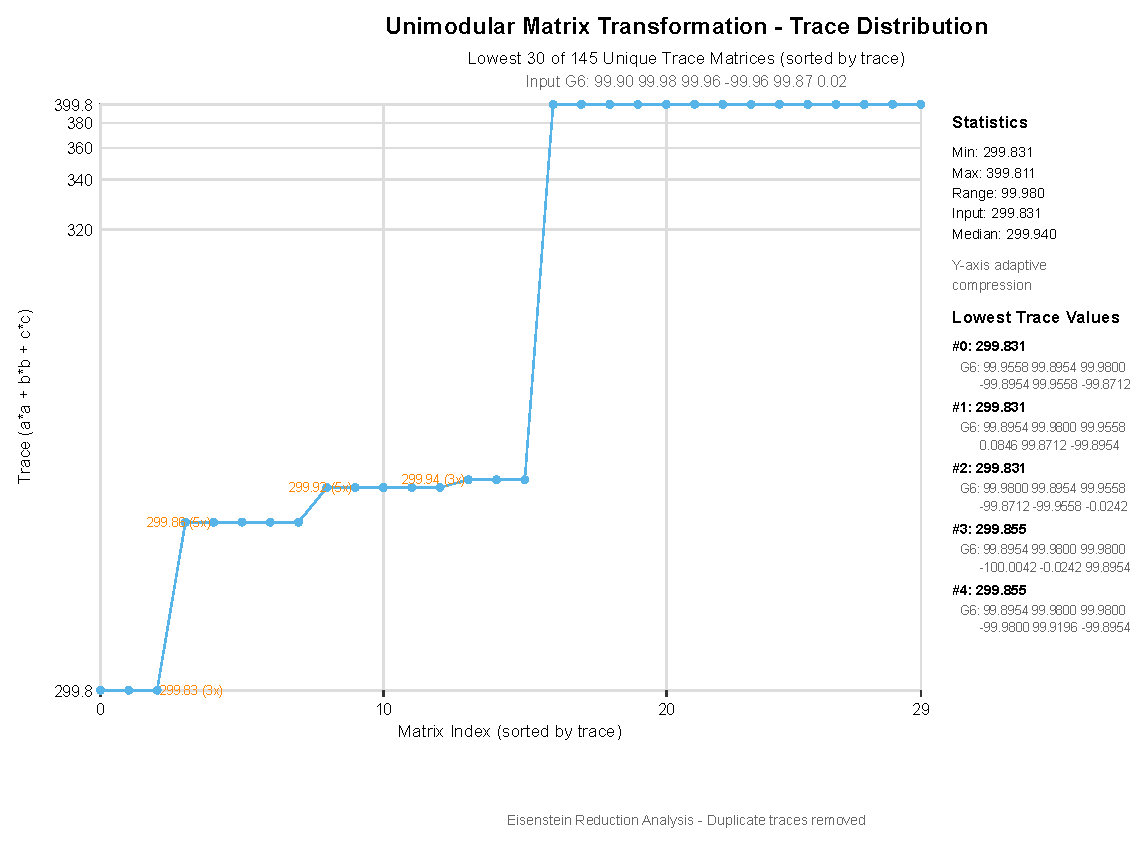
\includegraphics[width=\columnwidth]{PRR_2025-12-15.17_05_16_e774_1}
			\label{fig:trace}
			\caption{Trace distribution for the lowest 30 of 145 unimodular
				transforms of the input cell
				$G^6 = (99.90, 99.98, 99.96, -99.96, 99.87, 0.02)$.
				The three leftmost points share the global minimum trace of
				$299.831$; additional clusters at $299.855$, $299.921$,
				$299.940$ contain five, five, and three cells respectively.
				Niggli's secondary conditions select a unique reduced cell from
				among the degenerate trace-minimal candidates.}
		\end{center}
	\end{figure}
	
	
	\section{Examples}
	\label{sec:examples}
	
	% -----------------------------------------------------------------------
	% PLACEHOLDER: worked examples to be added
	% Each example should: give input cell parameters, show the G6 vector,
	% identify the minimum-trace cell(s), and show which Niggli secondary
	% condition resolves any degeneracy.
	% -----------------------------------------------------------------------
	
	\subsection{Example 1}
	
	[To be completed.]
	
	\subsection{Example 2}
	
	[To be completed.]
	
	
	\section{Summary}
	\label{sec:summary}
	
	Niggli reduction is most naturally understood as a two-stage process:
	first, minimize $\mathrm{Tr}(\mathbf{G}) = g_1 + g_2 + g_3$ to find
	the most compact cell; second, apply Niggli's ordering and
	sign-consistency conditions in \GVI{} to select a unique canonical
	representative from among all cells sharing the minimum trace. The
	secondary conditions are not optional refinements but are essential,
	because many distinct cells share the same minimum trace value.
	
	The termination argument of \citeasnoun{Krivy1976} is itself
	implicitly a trace-minimization argument: every step either decreases
	$\mathrm{Tr}(\mathbf{G})$ or is shown by case analysis to lead to a
	state that will. The stopping criterion of
	\citeasnoun{grosse2004numerically} for their minimum-reduction
	algorithm makes this explicit. The causes of infinite loops in
	floating-point implementations are distinct and enumerable:
	near-boundary floating-point oscillation, interaction between
	uniqueness steps, near-degeneracy of the trace minimum, and
	degenerate cell parameters. A maximum cycle count, simple and
	reliable, guards against all of them.
	
	
	\section{Availability of code}
	
	Reduction software and related tools are available at
	\url{https://github.com/duck10/LatticeRepLib.git}.
	
	
	\ack{{\bf Acknowledgements}}
	
	Careful copy-editing and corrections by Frances C. Bernstein are
	gratefully acknowledged.
	
	\ack{{\bf Funding information}}
	
	Funding for this research was provided in part by:
	U.S. Department of Energy Offices of Biological and
	Environmental Research and of Basic Energy Sciences
	(grant No. DE-AC02-98CH10886; grant No. E-SC0012704);
	U.S. National Institutes of Health (grant No. P41RR012408;
	grant No. P41GM103473; grant No. P41GM111244;
	grant No. R01GM117126,
	grant No. 1R21GM129570); Dectris, Ltd.
	
	
	\section{Synopsis}
	
	Niggli reduction is reframed as minimization of the trace of the metric
	tensor, with secondary conditions enforcing uniqueness. Multiple distinct
	unit cells can share the same minimum trace, and Niggli's conditions
	select a unique canonical representative from among them.
	
	
\appendix
\appendix

\section*{Appendix A. Local unimodular minimality implies the Niggli inequalities}

This appendix establishes that a primitive lattice basis which is locally
minimal under orientation–preserving unimodular transformations
automatically satisfies all Niggli inequalities, up to even permutations
and even sign changes of the basis vectors.  This provides a geometric
explanation for why the Niggli-reduced cell is the canonical
representative of a locally minimal basis.

\subsection*{A.1. Notation and assumptions}

Let $L \subset \mathbb{R}^3$ be a primitive lattice, and let


\[
B = [\,\mathbf{a}\ \mathbf{b}\ \mathbf{c}\,]
\]


be a basis matrix whose columns are the basis vectors.

Because $L$ is a primitive crystallographic lattice and chirality must be
preserved, we restrict attention to orientation–preserving unimodular
integer matrices:


\[
U \in \mathrm{SL}_3(\mathbb{Z}), \qquad \det U = +1.
\]


Applying $U$ gives another basis


\[
B' = B\,U,
\qquad
(\mathbf{a}',\mathbf{b}',\mathbf{c}') = (\mathbf{a},\mathbf{b},\mathbf{c})\,U.
\]



\paragraph{Local unimodular minimality.}
We assume that the basis is \emph{locally minimal} under all elementary
orientation–preserving unimodular transformations.  Concretely, this
means:

\begin{itemize}
	\item even permutations of $(\mathbf{a},\mathbf{b},\mathbf{c})$,
	\item elementary integer column operations such as
	$\mathbf{a} \mapsto \mathbf{a} \pm \mathbf{b}$,
	$\mathbf{b} \mapsto \mathbf{b} \pm \mathbf{c}$,
	$\mathbf{c} \mapsto \mathbf{c} \pm \mathbf{a}$,
	provided the resulting matrix lies in $\mathrm{SL}_3(\mathbb{Z})$,
	\item sign flips of basis vectors only when an even number of vectors
	are negated (or when combined with an even permutation) so that
	the resulting matrix remains in $\mathrm{SL}_3(\mathbb{Z})$.
\end{itemize}

Local minimality means that none of these allowed transformations
produces a strictly shorter replacement for the vector it modifies.
Equivalently, no allowed unimodular neighbor has a lexicographically
smaller metric tuple.

\paragraph{Metric notation.}
We use the standard $G^6$ metric representation:


\[
g_1 = \mathbf{a}\!\cdot\!\mathbf{a},\qquad
g_2 = \mathbf{b}\!\cdot\!\mathbf{b},\qquad
g_3 = \mathbf{c}\!\cdot\!\mathbf{c},
\]




\[
g_4 = 2\,\mathbf{b}\!\cdot\!\mathbf{c},\qquad
g_5 = 2\,\mathbf{a}\!\cdot\!\mathbf{c},\qquad
g_6 = 2\,\mathbf{a}\!\cdot\!\mathbf{b}.
\]


The factor of $2$ is conventional and matches the IUCr definition of the
$G^6$ metric.

Even permutations and even sign flips do not change the diagonal terms
and only change the signs of $g_4,g_5,g_6$.  These operations are used
only to select a canonical representative and do not affect minimality.



\appendix

\section*{Appendix B. Niggli inequalities as consequences of local unimodular minimality}
\label{app:niggli-from-local-min}

In this appendix we show that the standard Niggli inequalities follow
from a precise notion of \emph{local unimodular minimality} under
orientation–preserving basis changes.  Throughout, we work only with
transformations in $\mathrm{SL}_3(\mathbb{Z})$, so that chirality is
preserved.

\subsection*{B.1. Local unimodular minimality}

Let $(\mathbf{a},\mathbf{b},\mathbf{c})$ be a primitive basis of a
3-dimensional lattice, and let


\[
(g_1,g_2,g_3,g_4,g_5,g_6)
=
(a^2,b^2,c^2,2bc\cos\alpha,2ac\cos\beta,2ab\cos\gamma)
\]


be the associated metric parameters.  The diagonal terms
$g_1,g_2,g_3$ are squared lengths and therefore strictly positive.

\medskip

\noindent
\textbf{Allowed moves.}
We allow only orientation–preserving basis changes:


\[
U \in \mathrm{SL}_3(\mathbb{Z}), \qquad \det U = +1.
\]


These include:
\begin{itemize}
	\item even permutations of $(\mathbf{a},\mathbf{b},\mathbf{c})$,
	whose permutation matrices lie in $\mathrm{SL}_3(\mathbb{Z})$,
	\item elementary integer column operations such as
	$\mathbf{a} \mapsto \mathbf{a} \pm \mathbf{b}$,
	$\mathbf{b} \mapsto \mathbf{b} \pm \mathbf{c}$,
	etc., provided the resulting matrix lies in $\mathrm{SL}_3(\mathbb{Z})$,
	\item sign flips of basis vectors only when an \emph{even} number of
	vectors are negated (or when combined with an even permutation)
	so that the resulting matrix remains in $\mathrm{SL}_3(\mathbb{Z})$.
\end{itemize}
Only the off–diagonal terms $g_4,g_5,g_6$ may change sign under such
transformations.

\medskip

\noindent
\textbf{Objective function.}
We evaluate minimality using the standard Niggli objective


\[
\Phi(g_1,g_2,g_3,g_4,g_5,g_6)
=
(g_1,g_2,g_3,|g_4|,|g_5|,|g_6|)
\]


ordered lexicographically.  Absolute values appear only on the
off–diagonal terms because their signs may change under allowed basis
changes, whereas the diagonal terms are squared lengths and remain
strictly positive.

\medskip

\noindent
\textbf{Definition.}
A cell is \emph{locally unimodularly minimal} if for every allowed
$U \in \mathrm{SL}_3(\mathbb{Z})$,


\[
\Phi(g_1',\dots,g_6') \;\ge_{\mathrm{lex}}\; \Phi(g_1,\dots,g_6),
\]


where $(g_1',\dots,g_6')$ is the metric obtained from the transformed
basis.

\medskip

\noindent
Canonical sign conventions (e.g.\ $g_4 \le 0$) are not consequences of
minimality; they are imposed afterwards using transformations that do
not decrease $\Phi$.

\subsection*{B.2. Diagonal ordering $g_1 \le g_2 \le g_3$}

\paragraph{(1) $g_1 \le g_2$.}
Assume $g_2 < g_1$.  Consider the allowed even permutation


\[
(\mathbf{a},\mathbf{b},\mathbf{c})
\mapsto
(\mathbf{b},\mathbf{a},\mathbf{c}),
\]


whose matrix has determinant $+1$.  The transformed metric has


\[
g_1' = g_2 < g_1,
\]


so


\[
\Phi(g_1',\dots,g_6') <_{\mathrm{lex}} \Phi(g_1,\dots,g_6),
\]


contradicting local unimodular minimality.  Hence $g_1 \le g_2$.

\paragraph{(2) $g_2 \le g_3$.}
The same argument applied to the even permutation
$(\mathbf{a},\mathbf{b},\mathbf{c}) \mapsto (\mathbf{a},\mathbf{c},\mathbf{b})$
shows that $g_2 \le g_3$ must hold.

\medskip

\noindent
Thus local unimodular minimality forces


\[
g_1 \le g_2 \le g_3.
\]



\subsection*{B.3. Off–diagonal bounds}

We now show that the inequalities


\[
|g_4| \le g_2,\qquad |g_5| \le g_1,\qquad |g_6| \le g_1
\]


follow from local unimodular minimality.

\paragraph{(3) $|g_4| \le g_2$.}
Suppose $|g_4| > g_2$.  Consider the allowed transformation


\[
\mathbf{b}' = \mathbf{b} - \operatorname{sgn}(g_4)\,\mathbf{c},
\qquad
(\mathbf{a},\mathbf{b},\mathbf{c}) \mapsto (\mathbf{a},\mathbf{b}',\mathbf{c}),
\]


whose matrix lies in $\mathrm{SL}_3(\mathbb{Z})$.  Then


\[
\|\mathbf{b}'\|^2 = g_2 + g_3 - 2|g_4|.
\]


Since $|g_4| > g_2$ and $g_2 \le g_3$,


\[
\|\mathbf{b}'\|^2 < g_3.
\]



There are now three possibilities:
\begin{itemize}
	\item If $\|\mathbf{b}'\|^2 < g_1$, then after reordering by an even
	permutation the new diagonal triple begins with a strictly
	smaller first entry.
	\item If $g_1 \le \|\mathbf{b}'\|^2 < g_2$, then the new diagonal
	triple has a strictly smaller second entry.
	\item If $g_2 \le \|\mathbf{b}'\|^2 < g_3$, then the new diagonal
	triple has a strictly smaller third entry.
\end{itemize}
In all cases the objective $\Phi$ is lexicographically smaller,
contradicting minimality.  Hence $|g_4| \le g_2$.

\paragraph{(4) $|g_5| \le g_1$.}
If $|g_5| > g_1$, apply the allowed transformation


\[
\mathbf{a}' = \mathbf{a} - \operatorname{sgn}(g_5)\,\mathbf{c},
\]


whose matrix lies in $\mathrm{SL}_3(\mathbb{Z})$.  The same computation
shows that $\|\mathbf{a}'\|^2 < g_3$, and the same case analysis yields a
lexicographically smaller diagonal triple.  Thus $|g_5| \le g_1$.

\paragraph{(5) $|g_6| \le g_1$.}
The argument is identical, using
$\mathbf{a}' = \mathbf{a} - \operatorname{sgn}(g_6)\,\mathbf{b}$.

\subsection*{B.4. Sign conventions and tie–breaking}

The remaining Niggli conditions (sign conventions and tie–breaking
inequalities) do not follow from minimality; they select a canonical
representative among metrically equivalent minimal cells.

For example, if $g_4 > 0$ in a region where the convention requires
$g_4 \le 0$, the allowed transformation


\[
(\mathbf{a},\mathbf{b},\mathbf{c})
\mapsto
(\mathbf{a},-\mathbf{b},-\mathbf{c}),
\]


which has determinant $+1$, changes the sign of $g_4$ without altering
$\Phi$.  Thus sign conventions can be imposed without violating
minimality.

Similarly, when equalities such as $g_1 = g_2$ occur, Niggli’s
tie–breaking inequalities select one of several equally minimal cells.
These choices do not follow from minimality but are compatible with it.

\subsection*{B.5. Summary}

Local unimodular minimality under orientation–preserving basis changes
forces:


\[
g_1 \le g_2 \le g_3,\qquad
|g_4| \le g_2,\qquad
|g_5| \le g_1,\qquad
|g_6| \le g_1.
\]


The remaining Niggli conditions (sign conventions and tie–breakers)
select a canonical representative among equally minimal cells and are
compatible with, but not implied by, minimality.


	
	\bibliography{Reduced}
	
	\bibliographystyle{iucr}
	
\end{document}                    % DO NOT DELETE THIS LINE
%%%%%%%%%%%%%%%%%%%%%%%%%%%%%%%%%%%%%%%%%%%%%%%%%%%%%%%%%%%%%%%%%%%%%%%%%%%%%%